\chapter{Sistema de entrenamiento evolutivo} \label{chap:entrenador}

Una vez definida la arquitectura del agente autónomo en el capítulo anterior, el siguiente paso lógico es el proceso de optimización de los pesos que rigen su comportamiento. La función de evaluación del bot, aunque incorpora heurísticas y conocimiento experto, depende fundamentalmente del vector de pesos para ponderar la importancia de cada faceta del juego. Encontrar un conjunto de pesos óptimo para esta función es un problema de búsqueda en un espacio de soluciones de alta dimensionalidad, una tarea para la cual los algoritmos evolutivos están especialmente indicados. Este capítulo se dedica a describir en detalle al ``entrenador'': un sistema desarrollado en Python que orquesta un algoritmo evolutivo con el objetivo de encontrar el genoma (el conjunto de pesos) que maximice el rendimiento del bot. Se explorará su arquitectura general, los mecanismos de comunicación con el simulador, la implementación del algoritmo evolutivo utilizando la librería \textit{inspyred}, y las distintas estrategias de evaluación de fitness que se han diseñado e implementado.


\section{Arquitectura general del entrenador} \label{sec:arquitectura_entrenador}

El sistema de entrenamiento está formado por una serie de scripts modularizados y diseñados para ejecutar el proceso de optimización. Su objetivo final es determinar el conjunto de pesos más óptimo para la función de evaluación del agente descrito en el capítulo \ref{sec:definicion_pesos}. El sistema se apoya en la librería de código abierto \textit{inspyred} \cite{garrett_aarongarrettinspyred_2012}, un paquete que proporciona los componentes fundamentales del proceso, como la gestión de la población, los operadores de selección y variación, y el bucle evolutivo principal. Sobre esta base, se ha construido una arquitectura a medida que permite una extracción de datos mucho más granular, así como los modos de evaluación fijo, coevolutivo e híbrido y un sistema de ``salón de la fama'' generacional.

El flujo de trabajo del entrenador sigue el paradigma de un algoritmo evolutivo, operando a través de un ciclo iterativo de mejora generacional. El proceso comienza con la generación de una población inicial de individuos, donde cada individuo representa un ``genoma'' completo, es decir, un vector de 20 pesos aleatorios de 0.0 a 1.0. A partir de ahí, se inicia el bucle principal. En cada generación, se lleva a cabo la fase de ``evaluación'', donde cada individuo de la población es puesto a prueba. Para ello, el entrenador lanza una serie de partidas simuladas en el entorno de \textit{Scripts of Tribute}, pasando los pesos del individuo al bot. La tasa de victorias obtenida en estas partidas se convierte en la puntuación de \textit{fitness} de dicho individuo. Una vez que todos los individuos han sido evaluados, se aplica la fase de ``selección'', donde los individuos con mejor fitness se eligen para convertirse en los ``padres'' de la siguiente generación. Posteriormente, en la fase de ``variación'', estos padres se combinan mediante operadores de cruce y mutación para crear una nueva población de ``hijos''. Finalmente, se escogen los individuos con mayor \textit{fitness} y el ciclo vuelve a comenzar. Este proceso se repite hasta que se alcanza una condición de terminación, como un número máximo de evaluaciones, momento en el cual el mejor individuo que se haya encontrado a lo largo de toda la ejecución es proclamado como la solución más óptima encontrada. Como resumen de este proceso, en el algoritmo \ref{alg:proceso_evolutivo} se muestra el pseudocódigo del bucle evolutivo principal.

\begin{algorithm}[H]
	\caption{Proceso del Algoritmo Evolutivo}
	\label{alg:proceso_evolutivo}
	\begin{algorithmic}[1]
		\State \Comment{Orquestación del entrenamiento para optimizar los pesos del agente.}
		\State \textbf{Entradas:} Parámetros de configuración (tamaño de población $\mu$, máx. evaluaciones, etc.).
		\State
		\State $P \leftarrow \text{InicializarPoblaciónAleatoria}(\mu)$
		\State $H \leftarrow \emptyset$ \Comment{Inicializar Salón de la Fama interno.}
		\State $\text{Evaluar}(P, H)$
		\State
		\State \textbf{mientras} no se cumpla el criterio de parada \textbf{hacer}
		\State \quad $Padres \leftarrow \text{Seleccionar}(P)$
		\State \quad $Hijos \leftarrow \text{Variar}(Padres)$
		\State \quad $\text{Evaluar}(Hijos, H)$
		\State \quad $P \leftarrow \text{Reemplazar}(P, Hijos)$
		\State \quad $H \leftarrow \text{GestionarSalónDeLaFama}(P, H)$ \Comment{Algoritmo \ref{alg:hof_management}.}
		\State \textbf{fin mientras}
		\State
		\State \textbf{devolver} $\text{MejorIndividuo}(P \cup H)$
	\end{algorithmic}
\end{algorithm}


\section{El algoritmo evolutivo con Inspyred} \label{sec:algoritmo_evolutivo_inspyred}

El tipo de algoritmo evolutivo escogido para este trabajo sigue una Estrategia Evolutiva, concretamente la implementación canónica que proporciona la clase \texttt{inspyred.ec.ES} \cite{aaron_garret_library_2025}. Las estrategias evolutivas son especialmente adecuadas para problemas de optimización en espacios de búsqueda con valores reales, como es el caso de los 20 pesos que conforman el genoma del agente. La característica más notable de esta implementación es el uso de una mutación autoadaptativa, lo que significa que el genoma de cada individuo no solo contiene el vector de pesos de la solución, sino que también cuenta con un conjunto de ``parámetros de estrategia'' \cite{aaron_garret_library_2025}. Estos parámetros, uno por cada peso, funcionan como tasas de mutación individuales que evolucionan junto con la solución. De esta forma, el algoritmo no depende de una tasa de mutación global y fija, sino que aprende por sí mismo cómo de grande debe ser el paso de mutación para cada peso, permitiendo dar grandes saltos exploratorios en las primeras generaciones y ajustes más finos en las últimas. La librería gestiona este proceso de forma transparente, envolviendo automáticamente las funciones de generación y evaluación para añadir y quitar estos parámetros de estrategia sin necesidad de modificar la lógica específica del problema \cite{aaron_garret_library_2025}.

La configuración del algoritmo utiliza algunos de los componentes que la clase \texttt{inspyred.ec.ES} ofrece por defecto y otros personalizados para adaptarse a las necesidades del proyecto. A continuación se detallan sus componentes clave:
\begin{itemize}
	\item \textbf{Generador:} Se utiliza un método a medida, que crea un individuo con pesos aleatorios. La librería la envuelve con su propio generador para añadirle los parámetros de estrategia iniciales \cite{aaron_garret_library_2025}.
	\item \textbf{Evaluador:} Se emplean los orquestadores personalizados, que calculan la tasa de victorias. Internamente, \textit{inspyred} se asegura de que solo los pesos de la solución, y no los parámetros de estrategia, se pasen a esta función \cite{aaron_garret_library_2025}.
	\item \textbf{Selector:} Se utiliza la selección por defecto de la clase, que simplemente selecciona a toda la población para que actúen como padres en la siguiente generación \cite{aaron_garret_library_2025}.
	\item \textbf{Variador:} El operador de variación es un método interno de la clase \texttt{ES} que implementa la mutación gaussiana autoadaptativa. Primero modifica los parámetros de estrategia de cada individuo y luego los utiliza como la desviación estándar para aplicar una mutación gaussiana a los pesos de la solución \cite{aaron_garret_library_2025}.
	\item \textbf{Reemplazador:} Se emplea la estrategia de reemplazo por defecto, conocida como ``reemplazo $(\mu + \lambda)$''. En esta estrategia, la nueva generación se forma seleccionando a los mejores individuos del conjunto combinado de los padres de la generación actual y sus descendientes, asegurando que las mejores soluciones nunca se pierdan (como una forma de elitismo) \cite{aaron_garret_library_2025}.
\end{itemize}

A modo de resumen de la sección, en la figura \ref{fig:diagrama_algoritmo} se muestra un diagrama de flujo que ilustra el proceso del algoritmo evolutivo implementado con \textit{inspyred}.

\begin{figure}[H]
	\centering
	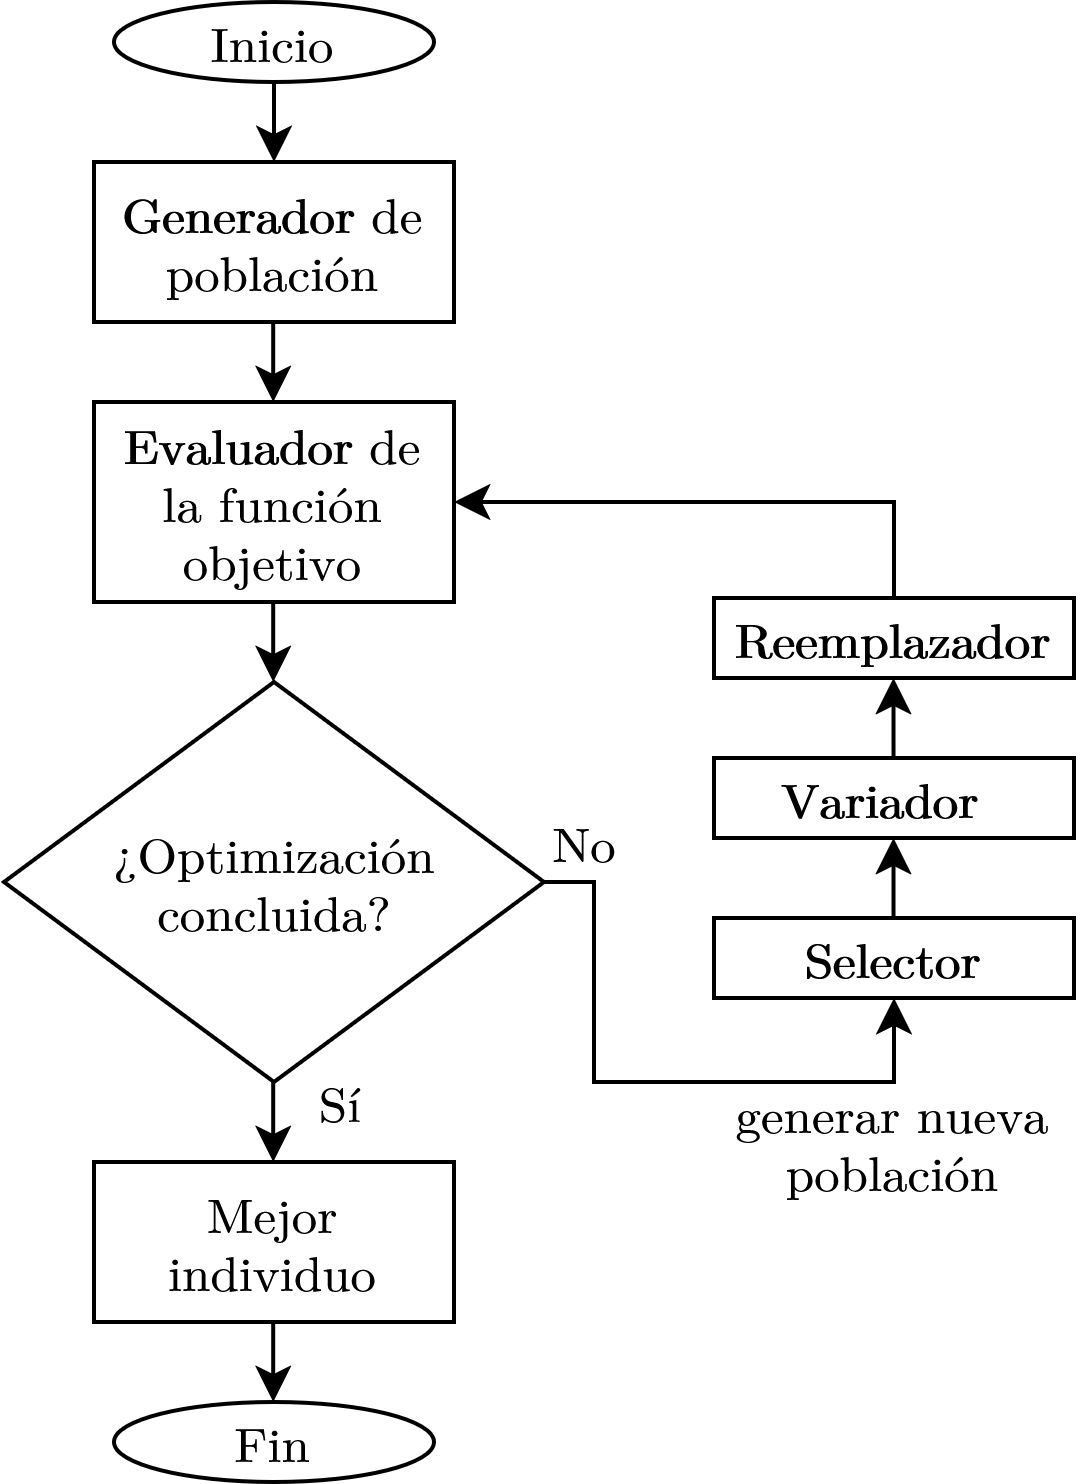
\includegraphics[width=0.6\textwidth]{img/diagrama_algoritmo.png}
	\caption{Diagrama del algoritmo evolutivo.}
	\label{fig:diagrama_algoritmo}
\end{figure}


\section{Comunicación entrenador-simulador} \label{sec:comunicacion_entrenador_simulador}

La arquitectura elegida para esta comunicación se basa en la creación de subprocesos. Por cada evaluación que el entrenador necesita realizar, el script de Python utiliza la librería \texttt{subprocess} para lanzar una nueva instancia del ejecutable \texttt{GameRunner}. Obviamente no lanza todos los procesos de la generación al mismo tiempo, si no que limita su creación al número de núcleos marcados por un argumento de entrada del entrenador. Este enfoque permite aislar cada simulación en su propio proceso y entorno. Una vez que el \texttt{GameRunner} finaliza su ejecución, escribe en su salida estándar (\textit{stdout}) un resumen de los resultados, como el número de victorias para cada jugador. El script de Python captura esta salida, la procesa para extraer los datos relevantes y así asigna una puntuación al individuo que estaba siendo evaluado.

Para la comunicación en sentido contrario se utiliza el método de variables de entorno ya descrito en el capítulo anterior. Más específicamente, antes de lanzar cada subproceso del \texttt{GameRunner}, entrenador realiza los siguientes pasos:
\begin{enumerate}
	\item Convierte el genoma del individuo en una única cadena de texto con los pesos separados por comas.
	\item Utiliza el módulo \texttt{os} de Python para establecer esta cadena como el valor de una variable de entorno específica.
	\item Lanza el subproceso del \texttt{GameRunner}, el cual hereda una copia del entorno del proceso padre, incluyendo la variable recién establecida.
\end{enumerate}

Al iniciarse la partida, el código del bot está programado para buscar y leer estas variables de entorno. Si las encuentra, procesa la cadena de texto para reconstruir el vector de pesos y se configura a sí mismo para la partida. Si no las encuentra, simplemente usa los pesos que lee desde un archivo de configuración que contiene los pesos del mejor individuo encontrado en el último experimento. Para garantizar la independencia de cada simulación, las variables de entorno se limpian y restauran a su estado original después de cada evaluación, evitando así que los pesos de un individuo se filtren accidentalmente en la evaluación del siguiente.

Como el sistema de gRPC no existía cuando se empezó a trabajar en el proyecto y se estimó que la funcionalidad brindada por la librería \textit{inspyred} era indispensable para el desarrollo del algoritmo evolutivo, se optó por esta solución de comunicación entre procesos, la cual se ha intentado mantener lo más eficiente posible dentro de las limitaciones de su arquitectura.


\section{El salón de la fama} \label{sec:salon_fama}

Uno de los problemas inherentes a los algoritmos evolutivos es el conocido como ``olvido catastrófico''. A medida que una población evoluciona durante muchas generaciones, su composición cambia. Puede especializarse en derrotar a sus contemporáneos inmediatos, pero al hacerlo, podría perder la capacidad de vencer a oponentes fuertes de generaciones muy anteriores, simplemente porque esos oponentes ya no existen en la población para ejercer presión selectiva. Para mitigar esta y otras patologías de la coevolución, una de las soluciones más extendidas es la implementación de un mecanismo de memoria a largo plazo \cite{mariela_nogueira_analysis_2013}. El sistema de ``salón de la fama'', implementado en este proyecto actúa como un archivo de campeones. Su función es preservar a los mejores individuos encontrados a lo largo de una misma carrera de entrenamiento\footnote{Una ``carrera'' o ``run'' es simplemente un proceso de optimización evolutiva desde la primera generación hasta la última. Un entrenamiento está compuesto por varias carreras.}. Al forzar a los nuevos candidatos a competir contra estos campeones del pasado, se intenta que el conocimiento estratégico no se degrade y que cualquier ``mejora'' sea un progreso genuino y no una simple especialización contra oponentes débiles. Este mecanismo, además, introduce una capa de dinámica coevolutiva incluso en el modo de entrenamiento fijo, ya que la población no solo se mide contra un baremo estático, sino también contra un conjunto de sus propios ancestros más capaces, los cuales van cambiando a lo largo del tiempo.

El diseño de este salón de la fama se inspira en las estrategias analizadas por Nogueira et al. en su trabajo sobre algoritmos coevolutivos competitivos del 2013 \cite{mariela_nogueira_analysis_2013}. En concreto, se ha implementado una variante de su estrategia \texttt{HofCC-Quality}. El objetivo de este enfoque es mantener en memoria únicamente a los individuos más capaces, eliminando periódicamente a los más débiles. En esta implementación, la ``debilidad'' de un campeón del salón de la fama se define por el número de derrotas que sufre contra la población de la generación actual. El sistema funciona bajo las siguientes reglas:

\begin{itemize}
	\item El salón de la fama mantiene un tamaño máximo configurable.
	\item Cuando se encuentra un nuevo campeón (un individuo con el mayor \textit{fitness} de su generación) y este no forma parte ya del salón de la fama, se considera su inclusión.
	\item Si el salón de la fama no está lleno, el nuevo campeón se añade directamente.
	\item Si el salón de la fama está lleno, el nuevo campeón debe ``desafiar'' al miembro más débil actualmente en el salón (aquel con más derrotas en la última generación). El nuevo campeón solo reemplazará al miembro existente si gana este enfrentamiento directo con una tasa de victorias superior al 50\%.
	\item Adicionalmente, para evitar el estancamiento, un mecanismo de ``poda'' se activa periódicamente cada cierto número de generaciones. Este proceso elimina un porcentaje configurable de los miembros más débiles del salón de la fama, forzando la renovación y asegurando que solo los contendientes más consistentemente fuertes permanezcan.
\end{itemize}

Esta lógica se puede resumir formalmente en el algoritmo \ref{alg:hof_management}.

\begin{algorithm}[H]
    \caption{Gestión del Salón de la Fama Interno}
    \label{alg:hof_management}
    \begin{algorithmic}[1]
        \State \Comment{Ejecutado al final de cada generación $g$, utilizando la población de supervivientes $P$.}
        \State \textbf{Entradas:} Población $P$, Salón de la Fama $H$, Generación actual $g$, Resultados detallados $D$.
        \State
        \State $\text{campeón} \leftarrow \text{MejorIndividuo}(P)$
        \State \textbf{si} $\text{ID}(\text{campeón}) \notin \text{IDs}(H)$ \textbf{entonces}
        \State \quad \textbf{si} $|H| < \text{tamaño\_máximo}$ \textbf{entonces}
        \State \qquad $H \leftarrow H \cup \{\text{campeón}\}$
        \State \quad \textbf{sino}
        \State \qquad \textbf{si} $\text{ID}(\text{campeón}) \in \text{Claves}(D)$ \textbf{entonces}
        \State \qquad \quad $\text{m\_débil} \leftarrow \text{MiembroMásDébil}(H, D)$
        \State \qquad \quad $\text{tasa\_victorias} \leftarrow \text{Enfrentar}(\text{campeón}, \text{m\_débil})$
        \State \qquad \quad \textbf{si} $\text{tasa\_victorias} > 0.5$ \textbf{entonces}
        \State \qquad \qquad $H \leftarrow (H \setminus \{\text{m\_débil}\}) \cup \{\text{campeón}\}$
        \State \qquad \quad \textbf{fin si}
        \State \qquad \textbf{fin si}
        \State \quad \textbf{fin si}
        \State \textbf{fin si}
        \State
        \State \Comment{Realizar la poda de forma periódica independientemente de si hubo un nuevo campeón.}
        \State \textbf{si} $g \pmod{\text{frecuencia\_poda}} = 0$ \textbf{entonces}
        \State \quad $\text{n\_poda} \leftarrow \lfloor |H| \cdot \text{porcentaje\_poda} \rfloor$
        \State \quad \textbf{si} $\text{n\_poda} > 0$ \textbf{entonces}
        \State \qquad $\text{H\_ordenado} \leftarrow \text{OrdenarPorDerrotas}(H)$
        \State \qquad $H \leftarrow \text{EliminarPeores}(\text{H\_ordenado}, \text{n\_poda})$
        \State \quad \textbf{fin si}
        \State \textbf{fin si}
    \end{algorithmic}
\end{algorithm}

En un principio se diseñó otro tipo salón de la fama, el cual abordaba el problema del olvido catastrófico de una forma diferente. En lugar de operar entre generaciones, operaba entre carreras. Este salón de la fama global almacenaba los campeones de cada carrera y los mantenía en memoria durante todo el ciclo de vida del entrenador para usarse en los siguientes entrenamientos. Sin embargo, este enfoque no era estadísticamente válido, ya que los campeones de una carrera no deberían afectar a los campeones de otra. Para generar resultados estadísticamente significativos, cada entrenamiento debe ser independiente y no influenciado por los resultados de otros. Por lo tanto, se optó por el salón de la fama interno detallado en esta sección.

\section{Arquitectura del orden, la evaluación y la paralelización} \label{sec:paralelizacion_algoritmo}

La fase de evaluación es, sin duda, el componente más crítico y costoso computacionalmente de cualquier algoritmo evolutivo. Para que el proceso de entrenamiento sea viable en un tiempo razonable, es imprescindible ejecutar las miles de simulaciones de partidas de forma lo más paralela posible. Para ello, se ha diseñado una arquitectura de evaluación basada en el módulo \texttt{concurrent.futures} de Python, que gestiona un conjunto de procesos trabajadores (\textit{workers}) para distribuir la carga de trabajo entre los múltiples núcleos de la CPU.

La comunicación del estado entre los procesos, como la gestión del salón de la fama interno, se gestiona utilizando objetos proxy proporcionados por la librería \texttt{multiprocessing.Manager}. Esta base tecnológica permite la implementación de diferentes ``orquestadores'' de evaluación, que son funciones de alto nivel encargadas de definir y distribuir las tareas específicas para cada una de las estrategias de fitness. La métrica de \textit{fitness} utilizada en todas ellas es la tasa de victorias normalizada, calculada como un porcentaje entre 0 y 100 para asegurar que los resultados sean comparables entre generaciones. Este nivel de personalización y sistemas específicos para el proyecto es necesario no solo para la implementación de los modos de evaluación, sino también para la correcta integración de otras características necesarias en el sistema. Por ejemplo, en el capítulo \ref{chap:plataforma_trabajo} se describió que el propio juego cuenta con una mecánica para nivelar la desventaja inherente al orden de los jugadores. Esta mecánica hace que el jugador que tiene su turno en segundo lugar empiece su turno con 1 moneda más. Incluso algo tan pequeño podría afectar a la tasa de victorias después de miles de partidas. Por eso, el sistema de evaluación se encarga de hacer que el bot juegue contra su oponente siendo primero un 50\% de las partidas y segundo el otro 50\%, y luego recoge acordemente el resultado de las partidas leyendo la salida estándar del \texttt{GameRunner}. Este tipo de características no podrían implementarse si use usase únicamente la librería \textit{inspyred} sin una capa de orquestación que gestione la comunicación y la lógica de evaluación.

\subsection{Modo fijo: evaluación contra oponentes estáticos} \label{sec:modo_fijo_evaluacion}

El modo fijo constituye el enfoque de evaluación más tradicional, donde el rendimiento de cada individuo se mide contra un conjunto estático de oponentes predefinidos. La lógica está encapsulada en la función orquestadora, que itera sobre la lista de candidatos a evaluar y, para cada uno, añade una tarea al conjunto de procesos. Cada tarea consiste en invocar a una función trabajadora que ejecuta una serie de partidas contra los bots de referencia de \textit{Scripts of Tribute} (ej. \texttt{PatronFavorsBot}) y contra los campeones del salón de la fama interno. En este caso, el orquestador evalúa únicamente al conjunto de hijos. Los padres de la generación anterior no son re-evaluados, ya que su \textit{fitness} contra un conjunto de oponentes estático no ha cambiado. Una vez finalizadas todas las simulaciones para un candidato, el trabajador devuelve su tasa de victorias, que el orquestador recoge para construir el vector de \textit{fitness} de la generación.

Formalmente, el \textit{fitness} para un individuo $i$ en modo fijo se calcula como su tasa de victorias global contra el conjunto de bots estáticos $B$ y el conjunto de campeones en el salón de la fama $H$, según la Ecuación \ref{eq:fitness_fijo}.

\begin{equation}
	\textit{Fitness}_{i} = \frac{\sum_{b \in B} v(i, b) + \sum_{h \in H} v(i, h)}{(|B| \cdot g_B) + (|H| \cdot g_H)} \cdot 100
	\label{eq:fitness_fijo}
\end{equation}

Donde $v(i, j)$ representa el número de victorias del individuo $i$ contra el oponente $j$. Los parámetros $|B|$ y $|H|$ son el número de bots estáticos y de miembros en el salón de la fama, respectivamente, mientras que $g_B$ y $g_H$ son el número de partidas jugadas contra cada tipo de oponente, tanto los fijos como los del salón de la fama.

\subsection{Modo coevolución: competición interna} \label{sec:modo_coevolucion_competicion}

La evaluación por coevolución, por su parte, mide la calidad de los individuos en relación a sus propios compañeros, creando una especie de ``carrera armamentística'' interna. En cada generación, se forma un ``conjunto de competición'' $P$, que consiste en la unión de los padres de la generación anterior y los hijos recién creados. A continuación, se genera una lista exhaustiva de enfrentamientos, que incluye partidas de todos contra todos (\textit{Round-robin}) entre los miembros de $P$, así como enfrentamientos de cada miembro de $P$ contra los campeones del salón de la fama $H$. Cada una de estas tareas se envía al conjunto de procesos para su ejecución en paralelo.

El cálculo del \textit{fitness} en este modo, aunque también es una tasa de victorias, se basa en un conjunto de oponentes completamente dinámico. La Ecuación \ref{eq:fitness_coevo} formaliza este cálculo.

\begin{equation}
	\textit{Fitness}_{i} = \frac{\sum_{p \in P, p \neq i} v(i, p) + \sum_{h \in H} v(i, h)}{(|P|-1) \cdot g_P + (|H| \cdot g_H)} \cdot 100
	\label{eq:fitness_coevo}
\end{equation}

Aquí, el sumatorio principal recorre a todos los demás individuos $p$ en el conjunto de competición $P$, y $v(i, p)$ son las victorias de $i$ contra ellos. El parámetro $g_P$ es el número de partidas por enfrentamiento entre pares. El componente del salón de la fama es idéntico al del modo fijo. Al final del proceso, el orquestador agrega todos los resultados para calcular la tasa de victorias final de cada individuo.

\subsection{Modo híbrido: combinando estrategias} \label{sec:modo_hibrido_combinando}

El modo híbrido se diseñó para combinar la guía inicial de conocimiento de los bots prexistentes del modo fijo con el potencial de innovación de la coevolución. Esta modalidad permite dividir una única carrera evolutiva en múltiples segmentos, cada uno con su propia estrategia de evaluación. El comportamiento se controla a través del parámetro \texttt{--hybrid\_schedule\_str}, que define la secuencia y duración relativa de cada segmento (ej. 40\% de fijo, 20\% de coevolución y otro 40\% de fijo). El bucle principal del entrenador es el responsable de interpretar este cronograma y de invocar dinámicamente al orquestador de evaluación correspondiente para cada fase de la evolución durante el número de generaciones adecuado.


\subsection{Análisis comparativo del coste computacional} \label{sec:comparativa_coste}

Como se ha descrito, los modos de evaluación fijo y de coevolución operan de formas muy distintas, lo que resulta en una diferencia sustancial en el coste computacional por cada generación. Para ilustrar este punto, a continuación se desglosa el número total de simulaciones de partidas requeridas por cada modo en una única generación. Es necesario aclarar que los valores totales dependen en gran medida de la configuración del experimento, como el número de partidas por enfrentamiento (tanto fijo como coevolutivo), el tamaño de la población o el número de miembros del salón de la fama. En este caso se han utilizado valores sencillos y representativos, pero que en algunos casos se ven incrementados para los experimentos finales.

\begin{itemize}
    \item \textbf{Coste en Modo Fijo:} En este modo, solo se evalúa a los 10 individuos ``hijos'' de la nueva generación. Cada uno de ellos se enfrenta al conjunto de oponentes estáticos y a los miembros del salón de la fama.
    \begin{itemize}
        \item \textit{Partidas contra bots estáticos:} 10 individuos $\times$ 3 bots $\times$ 10 partidas/bot = \textbf{300} partidas.
        \item \textit{Partidas contra el salón de la fama:} 10 individuos $\times$ 3 miembros del HoF $\times$ 3 partidas/miembro = \textbf{90} partidas.
        \item \textbf{Total por generación en modo fijo: 390 partidas.}
    \end{itemize}
    \vspace{0.5cm}
    
    \item \textbf{Coste en Modo Coevolución:} En este modo, el conjunto de la competición consta de 20 individuos (10 padres + 10 hijos), y todos ellos se enfrentan entre sí, además de contra el salón de la fama.
    \begin{itemize}
        \item \textit{Partidas Round-Robin:} El número de enfrentamientos únicos en un grupo de 20 es $\frac{20 \times 19}{2} = 190$ emparejamientos.
        \item 190 emparejamientos $\times$ 3 partidas/emparejamiento = \textbf{570} partidas.
        \item \textit{Partidas contra el salón de la fama:} 20 individuos $\times$ 3 miembros del HoF $\times$ 3 partidas/miembro = \textbf{180} partidas.
        \item \textbf{Total por generación en modo coevolución: 750 partidas.}
    \end{itemize}
\end{itemize}

Este pequeño cálculo demuestra que, a igualdad de tamaño de población, el modo de coevolución realiza aproximadamente el doble de partidas que el modo fijo. Aunque esto puede parecer un coste elevado, en el siguiente capítulo se verá que realmente las diferencias en el tiempo de entrenamiento no son tan significativas, sobretodo al utilizar el salón de la fama.

\section{Resumen de la arquitectura} \label{sec:resumen_architectura}

Para resumir la arquitectura del sistema de entrenamiento evolutivo, se ha diseñado un diagrama que ilustra los componentes principales y sus interacciones. La figura \ref{fig:diagrama_arquitectura} muestra cómo el entrenador se comunica con el simulador a través de subprocesos y este le devuelve los resultados de las partidas. Además, trata de representar las conexiones entre el entrenador, la librería \textit{inspyred} y la población de individuos, mostrando como el \textit{EvolutionaryBot} desarrollado en este proyecto los utiliza para guiar su función de evaluación.

\begin{figure}[H]
	\centering
	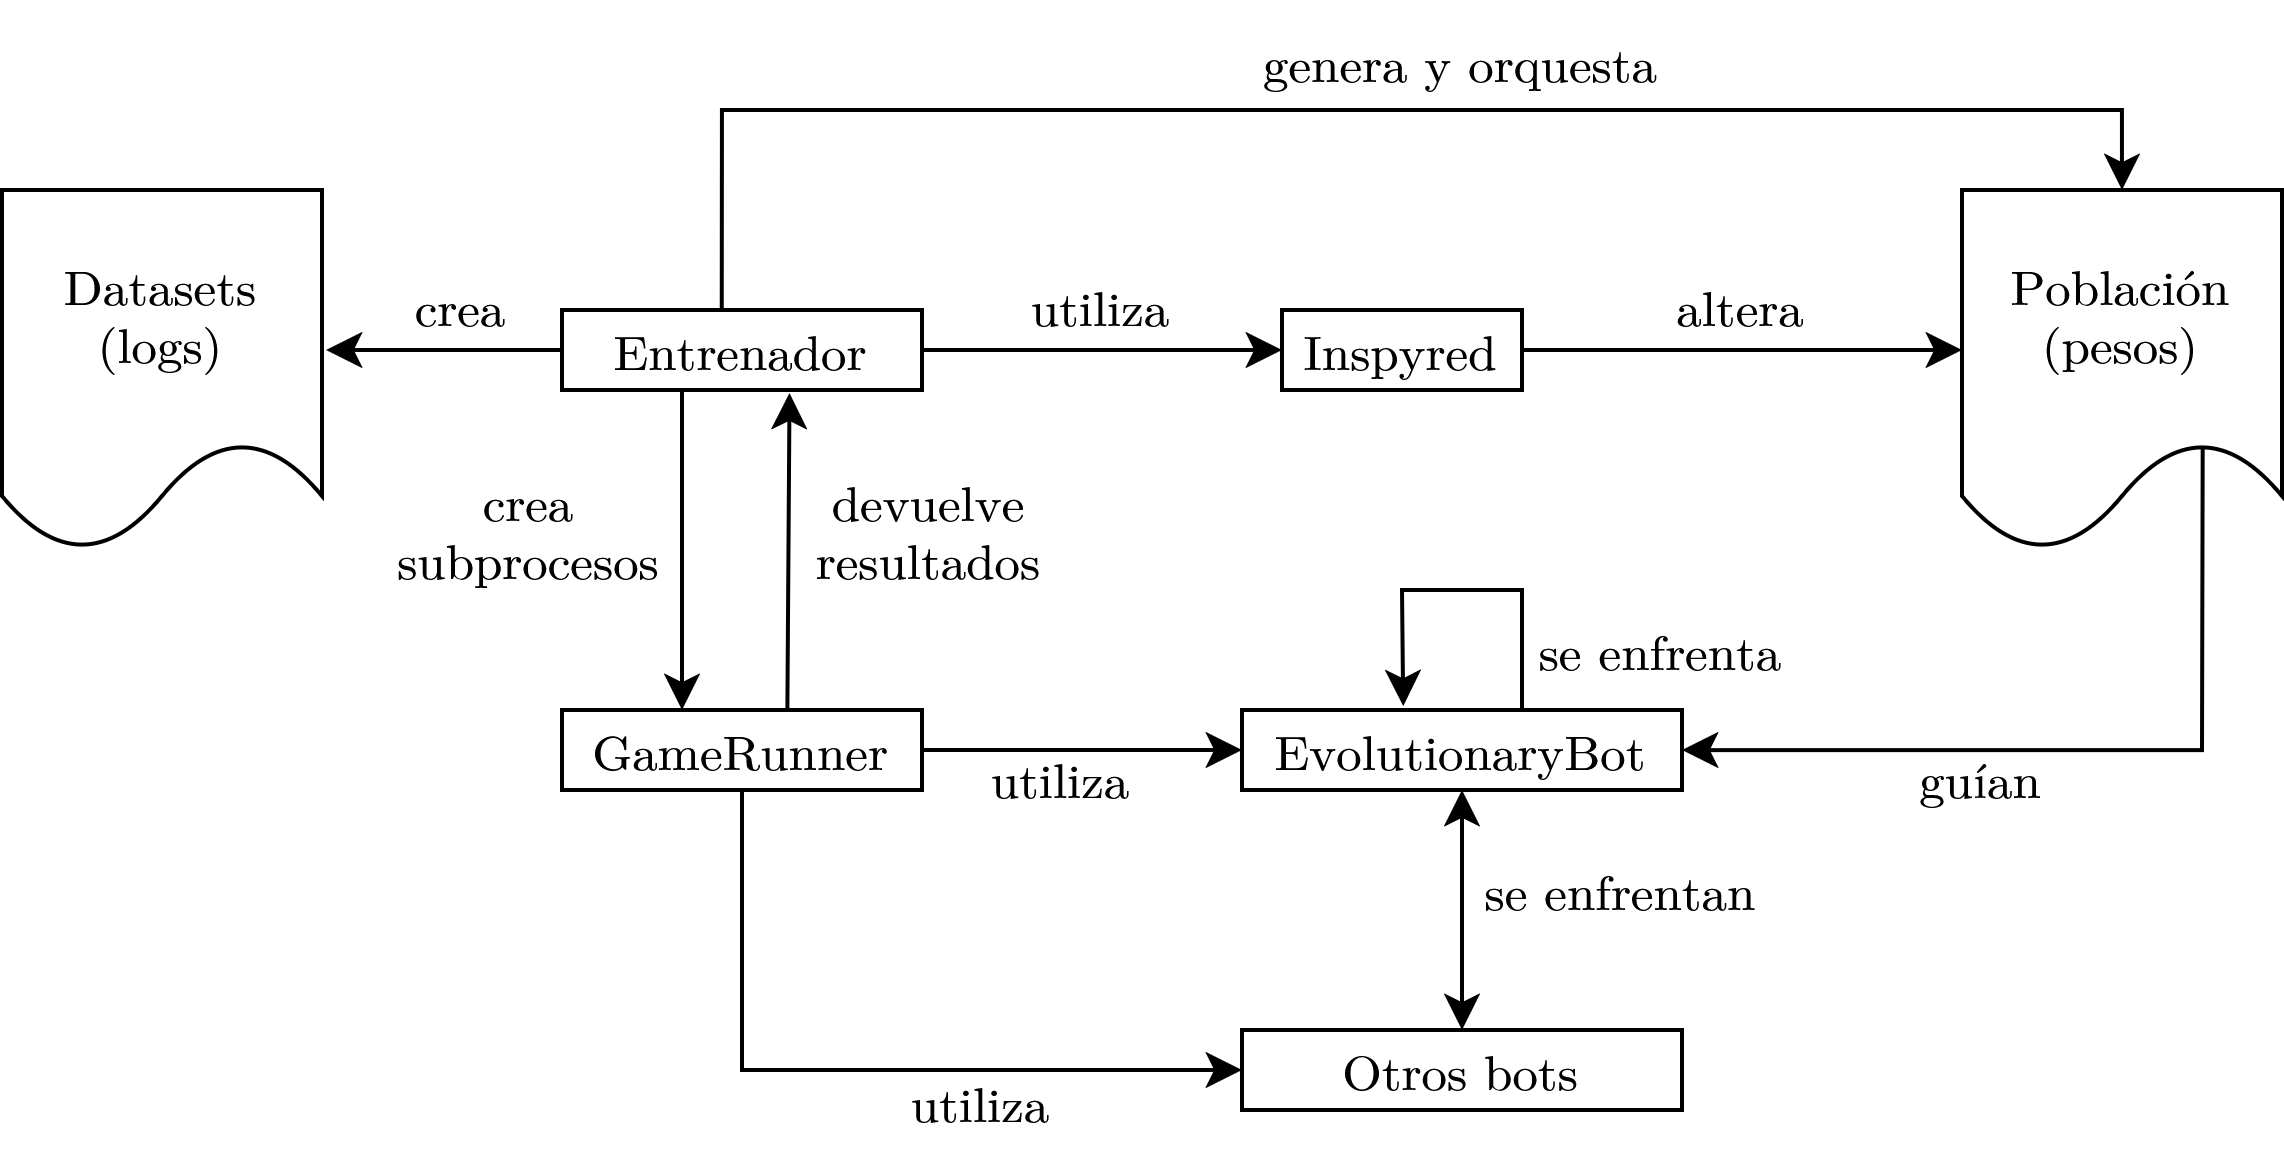
\includegraphics[width=1.0\textwidth]{img/diagrama_arquitectura.png}
	\caption{Diagrama de la arquitectura del proyecto.}
	\label{fig:diagrama_arquitectura}
\end{figure}

Este capítulo concluye el objetivo \textbf{OG3}, que consistía en desarrollar un programa de optimización en Python para ajustar los pesos de la función de fitness del agente, implementando y comparando dos estrategias principales: algoritmos coevolutivos y entrenamiento supervisado contra agentes de referencia de ``Scripts of Tribute''.